\documentclass[10pt]{beamer}\usepackage[]{graphicx}\usepackage[]{color}
% maxwidth is the original width if it is less than linewidth
% otherwise use linewidth (to make sure the graphics do not exceed the margin)
\makeatletter
\def\maxwidth{ %
  \ifdim\Gin@nat@width>\linewidth
    \linewidth
  \else
    \Gin@nat@width
  \fi
}
\makeatother

\definecolor{fgcolor}{rgb}{0.345, 0.345, 0.345}
\newcommand{\hlnum}[1]{\textcolor[rgb]{0.686,0.059,0.569}{#1}}%
\newcommand{\hlstr}[1]{\textcolor[rgb]{0.192,0.494,0.8}{#1}}%
\newcommand{\hlcom}[1]{\textcolor[rgb]{0.678,0.584,0.686}{\textit{#1}}}%
\newcommand{\hlopt}[1]{\textcolor[rgb]{0,0,0}{#1}}%
\newcommand{\hlstd}[1]{\textcolor[rgb]{0.345,0.345,0.345}{#1}}%
\newcommand{\hlkwa}[1]{\textcolor[rgb]{0.161,0.373,0.58}{\textbf{#1}}}%
\newcommand{\hlkwb}[1]{\textcolor[rgb]{0.69,0.353,0.396}{#1}}%
\newcommand{\hlkwc}[1]{\textcolor[rgb]{0.333,0.667,0.333}{#1}}%
\newcommand{\hlkwd}[1]{\textcolor[rgb]{0.737,0.353,0.396}{\textbf{#1}}}%
\let\hlipl\hlkwb

\usepackage{framed}
\makeatletter
\newenvironment{kframe}{%
 \def\at@end@of@kframe{}%
 \ifinner\ifhmode%
  \def\at@end@of@kframe{\end{minipage}}%
  \begin{minipage}{\columnwidth}%
 \fi\fi%
 \def\FrameCommand##1{\hskip\@totalleftmargin \hskip-\fboxsep
 \colorbox{shadecolor}{##1}\hskip-\fboxsep
     % There is no \\@totalrightmargin, so:
     \hskip-\linewidth \hskip-\@totalleftmargin \hskip\columnwidth}%
 \MakeFramed {\advance\hsize-\width
   \@totalleftmargin\z@ \linewidth\hsize
   \@setminipage}}%
 {\par\unskip\endMakeFramed%
 \at@end@of@kframe}
\makeatother

\definecolor{shadecolor}{rgb}{.97, .97, .97}
\definecolor{messagecolor}{rgb}{0, 0, 0}
\definecolor{warningcolor}{rgb}{1, 0, 1}
\definecolor{errorcolor}{rgb}{1, 0, 0}
\newenvironment{knitrout}{}{} % an empty environment to be redefined in TeX

\usepackage{alltt}


%\input{slides_header.tex}
\usepackage{graphicx}
\usepackage{hyperref, url}
\hypersetup{colorlinks,citecolor=myorange,filecolor=red,linkcolor=brown,urlcolor=blue}

\usepackage{longtable,booktabs}
\usepackage{amssymb,amsmath}
\usepackage{animate}
\usepackage{subfig}
\usepackage{tikz}
\usetikzlibrary{shapes.geometric, arrows,shapes.symbols,decorations.pathreplacing}
\tikzstyle{startstop} = [rectangle, rounded corners, minimum width=3cm, minimum height=1cm, draw=black, fill=pinkish,text width=3.5cm]
\tikzstyle{startstop2} = [rectangle, rounded corners, minimum width=3cm, minimum height=1cm, draw=black, fill=background,text width=4.5cm]
\tikzstyle{startstop3} = [rectangle, rounded corners, minimum width=3cm, minimum height=1cm, draw=black, fill=beige,text width=3.0cm]
\tikzstyle{startstop4} = [rectangle, rounded corners, minimum width=3cm, minimum height=1cm, draw=black, fill=pinkish,text width=4.5cm]
\tikzstyle{io} = [trapezium, trapezium left angle=70, trapezium right angle=110, minimum width=2cm, minimum height=1cm, text centered, draw=black, fill=blue!30,text width=1.5cm]
\tikzstyle{process} = [rectangle, minimum width=1cm, minimum height=1cm, text centered, draw=black, fill=orange!30,text width=2cm]
\tikzstyle{decision} = [diamond, minimum width=2cm, minimum height=1cm, text centered, draw=black, fill=green!30]
\tikzstyle{arrow} = [thick,->,>=stealth]
\tikzstyle{both} = [thick,<->,>=stealth, red]


% used for tree of stats tests in 001-introduction
\tikzstyle{startstopstats} = [rectangle, rounded corners, minimum width=2cm, minimum height=.5cm,text centered, draw=black, fill=red!30]
\tikzstyle{iostats} = [trapezium, trapezium left angle=70, trapezium right angle=110, minimum width=2cm, minimum height=.5cm, text centered, draw=black, fill=blue!30]
\tikzstyle{processstats} = [rectangle, minimum width=1.5cm, minimum height=.5cm, text centered, draw=black, fill=orange!30]
\tikzstyle{processbigstats} = [rectangle, minimum width=1.5cm, minimum height=.5cm, text centered, draw=black, fill=orange!30,text width=1.6cm]
\tikzstyle{decisionstats} = [rectangle, minimum width=1cm, minimum height=1cm, text centered, draw=black, fill=green!30,text width=1.6cm]
\tikzstyle{decisionbigstats} = [rectangle, minimum width=1cm, minimum height=1cm, text centered, draw=black, fill=yellow!30,text width=2cm]

\usepackage{pifont}% http://ctan.org/pkg/pifont
\newcommand{\cmark}{\ding{51}}%
\newcommand{\xmark}{\ding{55}}%

\usepackage{ulem} % for strikeout

\usepackage{xcolor}
\usepackage{color, colortbl}
\definecolor{lightgray}{RGB}{200,200,200}
\definecolor{palegray}{RGB}{221,221,221}
\definecolor{myblue}{RGB}{0,89,179}
\definecolor{myorange}{rgb}{0.776,0.357,0.157}
\definecolor{gray}{RGB}{110,110,110}
\definecolor{darkgray}{RGB}{100,100,100}
\definecolor{lightgray}{RGB}{200,200,200}
\definecolor{palegray}{RGB}{221,221,221}
\definecolor{turquoise}{RGB}{81,193,188}
\definecolor{tomato}{RGB}{255,136,136}
\definecolor{mandarina}{RGB}{229,169,25}
\definecolor{foreground}{RGB}{81,141,193}
\definecolor{background}{RGB}{246,244,240}
\definecolor{highlight}{RGB}{229,169,25}
\definecolor{lowlight}{RGB}{200,200,200}
\definecolor{beige}{RGB}{255,255,240}
\definecolor{pinkish}{RGB}{255,223,247}
\definecolor{darktangerine}{rgb}{1.0, 0.66, 0.07}
\definecolor{deepink}{RGB}{255,20,147}
%\usepackage{shadethm}
%\colorlet{shadecolor}{blue!15}
%\colorlet{shadecolor}{palegray}
%\setlength{\shadeboxrule}{.4pt}

%\newshadetheorem{thm}{Theorem}
%\newshadetheorem{defm}{Definition}
%\newshadetheorem{exm}{Exercise}
%\newshadetheorem{remarkm}{Remark}
%\definecolor{shadethmcolor}{HTML}{EDF8FF}
%\definecolor{shadethmcolor}{RGB}{221,221,221}
%\definecolor{shaderulecolor}{HTML}{45CFFF}
%\definecolor{shaderulecolor}{RGB}{0,89,179}
%\setlength{\shadeboxrule}{.4pt}



\usepackage{epsfig}

\newcommand{\code}[1]{\texttt{#1}}
\newcommand{\blue}[1]{\textcolor{blue}{#1}}
\newcommand{\red}[1]{\textcolor{red}{#1}}

\usepackage{comment}

\makeatletter

\def \iqsssectiontitleheader {}

\newcommand{\iqsssectiontitle}[1]{
	\def \iqsssectiontitleheader{#1}
}

\@ifundefined{insertmainframenumber}
{%
	% \insertmainframenumber not defined
	\newcommand{\insertmainframenumber}{\inserttotalframenumber}
}
{%
	% \insertmainframenumber already defined
}%


\AtBeginSection[]{
	\title{\insertsectionhead}
	{
		%\definecolor{white}{RGB}{140,193,250}
		%\definecolor{white}{RGB}{200,200,200}
		%\definecolor{white}{RGB}{242,244,247}
		\definecolor{white}{RGB}{0,89,179}
		%\definecolor{iqss@orange}{rgb}{1,1,1}
		\ifnum \insertmainframenumber > \insertframenumber
		%\setbeamercolor{background canvas}{bg=myblue}
		%\setbeamercolor{normal text}{fg=black,bg=white}
		%\setbeamercolor{frametitle}{fg=red}
		%\setbeamercolor{section in toc}{fg=myblue, bg=white}
		%\setbeamercolor{subsection in toc}{fg=myblue, bg=white}
		\frame{
			\frametitle{\iqsssectiontitleheader}
			\tableofcontents[currentsection]
		}
		\else
		\frame{
			\frametitle{Backup Slides}
			\tableofcontents[sectionstyle=shaded/shaded,subsectionstyle=shaded/shaded/shaded]
		}
		\fi
	}
}
\makeatother
%\graphicspath{{/home/sahir/git_repositories/EPIB607/resources/assets/slides/figure/}}


\usepackage{fontspec}
%\setsansfont{Fira Sans}
%\setmonofont{Fira Mono}
%\setsansfont[ItalicFont={Fira Sans Light Italic},BoldFont={Fira Sans},BoldItalicFont={Fira Sans Italic}]{Fira Sans Light}
%\setmonofont[BoldFont={Fira Mono Medium}]{Fira Mono}

\def\installpath{/usr/local/share/texmf/fonts/opentype/libertinus/}
\setmainfont{LibertinusSerif}[
UprightFont    = *-Regular,
BoldFont       = *-Bold,
ItalicFont     = *-Italic,
BoldItalicFont = *-BoldItalic,
Ligatures      = TeX,
Extension      = .otf,
Path           = \installpath/
]

\setsansfont{LibertinusSerif}[
UprightFont    = *-Regular,
BoldFont       = *-Bold,
ItalicFont     = *-Italic,
BoldItalicFont = *-BoldItalic,
Ligatures      = TeX,
Extension      = .otf,
Path           = \installpath/
]


%\setmonofont{LibertinusSerif}[
%UprightFont    = *-Regular,
%BoldFont       = *-Bold,
%ItalicFont     = *-Italic,
%BoldItalicFont = *-BoldItalic,
%Ligatures      = TeX,
%Extension      = .otf,
%Path           = \installpath/
%]






\newcommand\Wider[2][3em]{%
	\makebox[\linewidth][c]{%
		\begin{minipage}{\dimexpr\textwidth+#1\relax}
			\raggedright#2
		\end{minipage}%
	}%
}


\newcommand {\framedgraphic}[1] {
	\begin{figure}
		\centering
		\includegraphics[width=\textwidth,height=0.9\textheight,keepaspectratio]{#1}
	\end{figure}
}


\newcommand {\framedgraphiccaption}[2] {
	\begin{figure}
		\centering
		\includegraphics[width=\textwidth,height=0.8\textheight,keepaspectratio]{#1}
		\caption{#2}
	\end{figure}
}




\setbeamercolor{itemize item}{fg=myblue}
\setbeamercolor{itemize subitem}{fg=myorange}
%\setbeamertemplate{itemize item}[square]
\setbeamertemplate{itemize item}[circle]
\setbeamertemplate{itemize subitem}[triangle]
\setbeamertemplate{blocks}[rounded][shadow=true]
\setbeamercolor{block body alerted}{bg=alerted text.fg!10}
\setbeamercolor{block title alerted}{bg=alerted text.fg!20}
\setbeamercolor{block body}{bg=structure!10}
\setbeamercolor{block title}{bg=structure!20}
\setbeamercolor{block body example}{bg=green!10}
\setbeamercolor{block title example}{bg=green!20}


\makeatletter
\newenvironment<>{proofs}[1][\proofname]{%
	\par
	\def\insertproofname{#1\@addpunct{.}}%
	\usebeamertemplate{proof begin}#2}
{\usebeamertemplate{proof end}}
\newenvironment<>{proofc}{%
	\setbeamertemplate{proof begin}{\begin{block}{}}
		\par
		\usebeamertemplate{proof begin}}
	{\usebeamertemplate{proof end}}
	\newenvironment<>{proofe}{%
		\par
		\pushQED{\qed}
		\setbeamertemplate{proof begin}{\begin{block}{}}
			\usebeamertemplate{proof begin}}
		{\popQED\usebeamertemplate{proof end}}
\makeatother


\makeatletter
\newenvironment<>{exams}[1][\proofname]{%
	\par
	\def\insertproofname{#1\@addpunct{.}}%
	\usebeamertemplate{example begin}#2}
{\usebeamertemplate{example end}}
\newenvironment<>{examc}{%
	\setbeamertemplate{exam begin}{\begin{block}{}}
		\par
		\usebeamertemplate{exam begin}}
	{\usebeamertemplate{exam end}}
	\newenvironment<>{exame}{%
		\par
		\pushQED{\qed}
		\setbeamertemplate{exam begin}{\begin{block}{}}
			\usebeamertemplate{exam begin}}
		{\popQED\usebeamertemplate{exam end}}
		\makeatother

%\definecolor{mycolor}{HTML}{F7F8E0}
%\declaretheorem[shaded={bgcolor=mandarina}]{theo}
%\declaretheorem[shaded={bgcolor=mycolor}]{propo}
%\declaretheorem[shaded={bgcolor=green!80!black!30}]{remark}

%\setbeamertemplate{navigation symbols}{\usebeamercolor[fg]{title in head/foot}\usebeamerfont{title in head/foot}\insertframenumber}


%\setbeamertemplate{footline}{}

\beamertemplatenavigationsymbolsempty % toggle off if you want navigation symbols at the bottom

\setbeamertemplate{footline}
{ \usebeamercolor[fg]{page number in head/foot}%
	\usebeamerfont{page number in head/foot}%
	\hspace{1em}\insertsectionhead%
	\hfill%
	\insertframenumber\,/\,\hyperlinkappendixstart{\insertmainframenumber}
	\ifnum \thepage = \insertframeendpage{\small .}\else{\phantom{\small .}}\fi
	\hspace{1em}
	\vskip2pt%
}

%\newtheorem{proposition}[theorem]{Proposition}
%\newtheorem{exercise}[theorem]{Exercise}
%\newtheorem{remark}[theorem]{Remark}


\usepackage{amsthm}
\usepackage{thmtools}

\setbeamertemplate{theorems}[ams style] 
%\setbeamertemplate{theorems}[numbered] 
%\setbeamertemplate{corollary}[numbered] 
\newtheorem{proposition}{Proposition}
\newtheorem{exercise}{Exercise}
\newtheorem{remark}{Remark}
\newtheorem{exam}{Example}
%\newtheorem{proof}{Proof}
%\newtheorem{corollaries}[theorem]{Corollary}
\newcommand*{\theorembreak}{\usebeamertemplate{theorem end}\framebreak\usebeamertemplate{theorem begin}}



\setlength{\emergencystretch}{3em} % prevent overfull lines
\providecommand{\tightlist}{%
	\setlength{\itemsep}{0pt}\setlength{\parskip}{0pt}}

\newcommand\AddButton{%
	\setbeamertemplate{background canvas}{%
		\begin{tikzpicture}[remember picture,overlay]
		\node[anchor=west] at ([yshift=5pt,xshift=0.1em]current page.south west)
		{\hyperlink{toc}{\beamergotobutton{back to TOC}}};
		\end{tikzpicture}%
	}%
}


\titlegraphic{\hfill
\includegraphics[height=1cm]{/home/sahir/git_repositories/EPIB607/slides/mcgill_logo.png}}




\graphicspath{{/home/sahir/git_repositories/EPIB607/slides/figure/}}

%\let\oldShaded\Shaded
%\let\endoldShaded\endShaded
%\renewenvironment{Shaded}{\footnotesize\oldShaded}{\endoldShaded}

\newcommand{\blue}[1]{\textcolor{blue}{#1}}
\newcommand{\red}[1]{\textcolor{red}{#1}}


\usepackage{xparse}
\NewDocumentCommand\mylist{>{\SplitList{;}}m}
{
	\begin{itemize}
		\ProcessList{#1}{ \insertitem }
	\end{itemize}
}
\NewDocumentCommand\mynum{>{\SplitList{;}}m}
{
	\begin{enumerate}
		\ProcessList{#1}{ \insertitem }
	\end{enumerate}
}
\newcommand\insertitem[1]{\item #1}

\newcommand\FrameText[1]{%
	\begin{textblock*}{\paperwidth}(0pt,\textheight)
		\raggedright #1\hspace{.5em}
\end{textblock*}}
\IfFileExists{upquote.sty}{\usepackage{upquote}}{}
\begin{document}

	

%\title{Introduction to Regression Trees}
%\author{Sahir Bhatnagar \inst{1}}
%\author[shortname]{Sahir Rai Bhatnagar, PhD Candidate (Biostatistics) }
%\institute[shortinst]{Department of Epidemiology, Biostatistics and Occupational Health}

	\title{012 - $p$-values}
\author{EPIB 607 - FALL 2020}
\institute{
	Sahir Rai Bhatnagar\\
	Department of Epidemiology, Biostatistics, and Occupational Health\\
	McGill University\\
	
	\vspace{0.1 in}
	
	\texttt{sahir.bhatnagar@mcgill.ca}\\
	%\texttt{\url{https://sahirbhatnagar.com/EPIB607/}}
}

\date{slides compiled on \today}

\maketitle

\section{$p$-values}
\begin{frame}
	\frametitle{$p$-values and statistical tests}
	
	
	%\vspace{18pt}
	\begin{defm}[$p$-value]
		A \textbf{probability concerning the observed data}, calculated under a \textbf{Null Hypothesis} assumption, i.e., assuming that the only factor operating is sampling or measurement variation. 
	\end{defm}
	
	\begin{itemize} 
		\item[\underline{Use}] To assess the evidence provided by the sample data
		in relation to a pre-specified claim or `hypothesis' concerning some parameter(s) or data-generating process. 
		\item[\underline{Basis}] As with a confidence interval, it makes use of the concept of a \textit{distribution}. 
		\item[\underline{Caution}] A $p$-value is NOT the probability that the null `hypothesis' is true
	\end{itemize}
\end{frame}


\begin{frame}
	
	\frametitle{Example 1 -- from \textit{Design of Experiments}, by R.A. Fisher}
	
	\parindent 128pt
	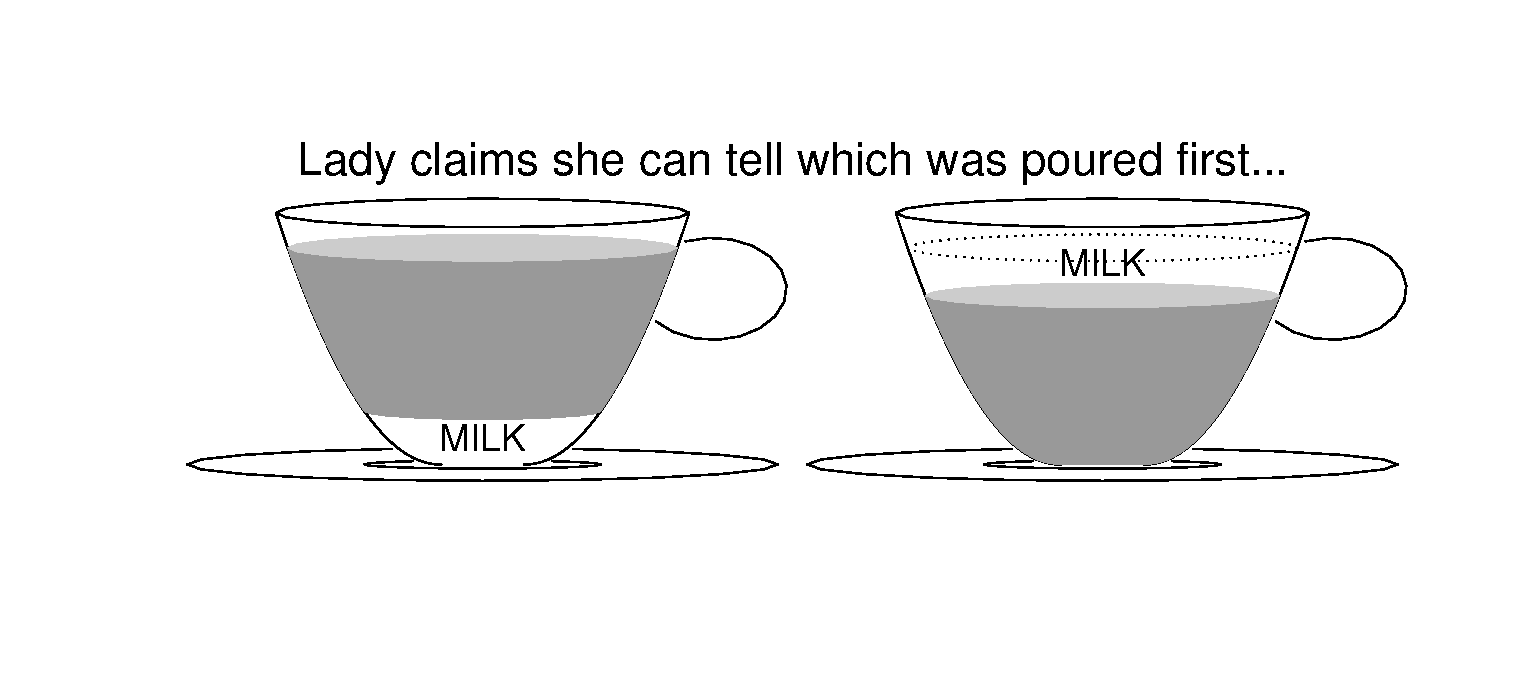
\includegraphics[width=1.8in]{TeaClaim.pdf}
	\parindent 0pt
	
	\begin{center}
		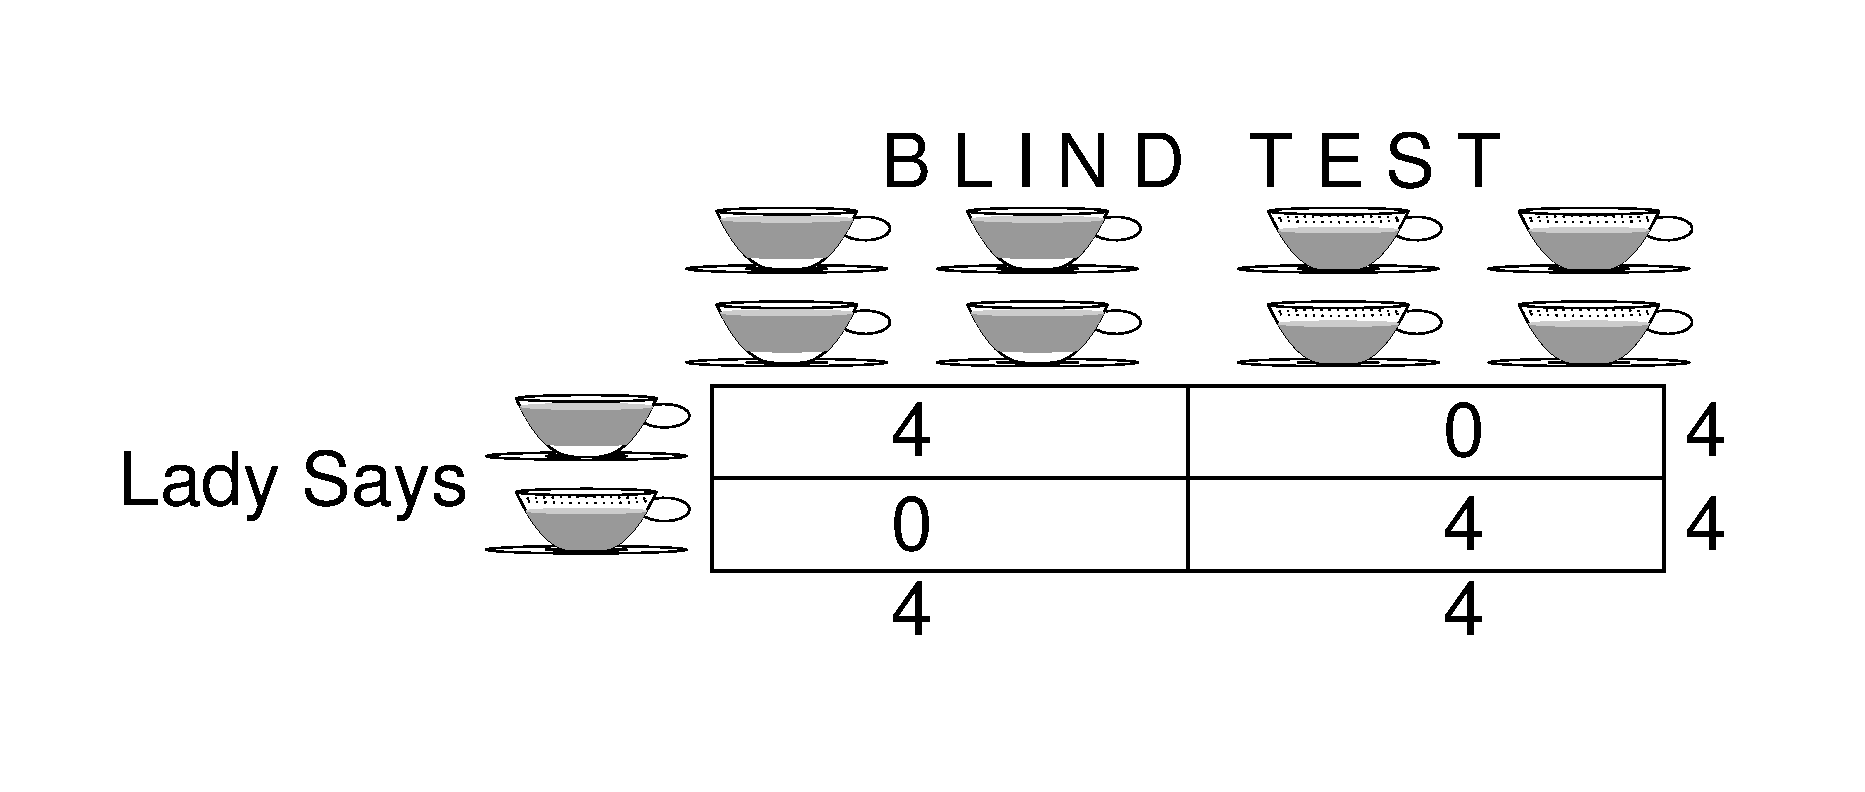
\includegraphics[width=3in]{BlindTest.pdf}
	\end{center}
	\blue{Null Hypothesis (H$_{null}$)}: she can not tell them apart, i.e., just guessing. \\ \ \\
	\blue{Alternative Hypothesis (H$_{alt}$)}: she can. \\ \ \\ \pause
	
	%\begin{scriptsize}
	%	Blind test is equivalent to
	%	being asked to say \textbf{which 4} of the following 8 Gaelic words  are the \textbf{correctly spelled}
	%	ones. You are told that \textbf{4 are correctly spelled \& 4 are not}. 
	%	\begin{center}
	%		\begin{tabular}{c c c c  c c c c}
	%			1&2&3&4&5&6&7&8\\
	%			madra&olscoil&cathiar&tanga&doras&cluicha&f\'ear&b\'othar \\
	%		\end{tabular}
	%	\end{center} 
	%\end{scriptsize}
	
	
\end{frame}

\begin{frame}
	\frametitle{The evidence provided by the test}
	
	\begin{footnotesize}
		\begin{itemize}
			\item
			Rank possible test
			results by  degree of evidence against H$_{null}$. 
			\item ``$p$-value'' is the probability, calculated under null hypothesis, of
			observing a result as  extreme as, or more extreme than, the one that was obtained/observed.
			\begin{center}
				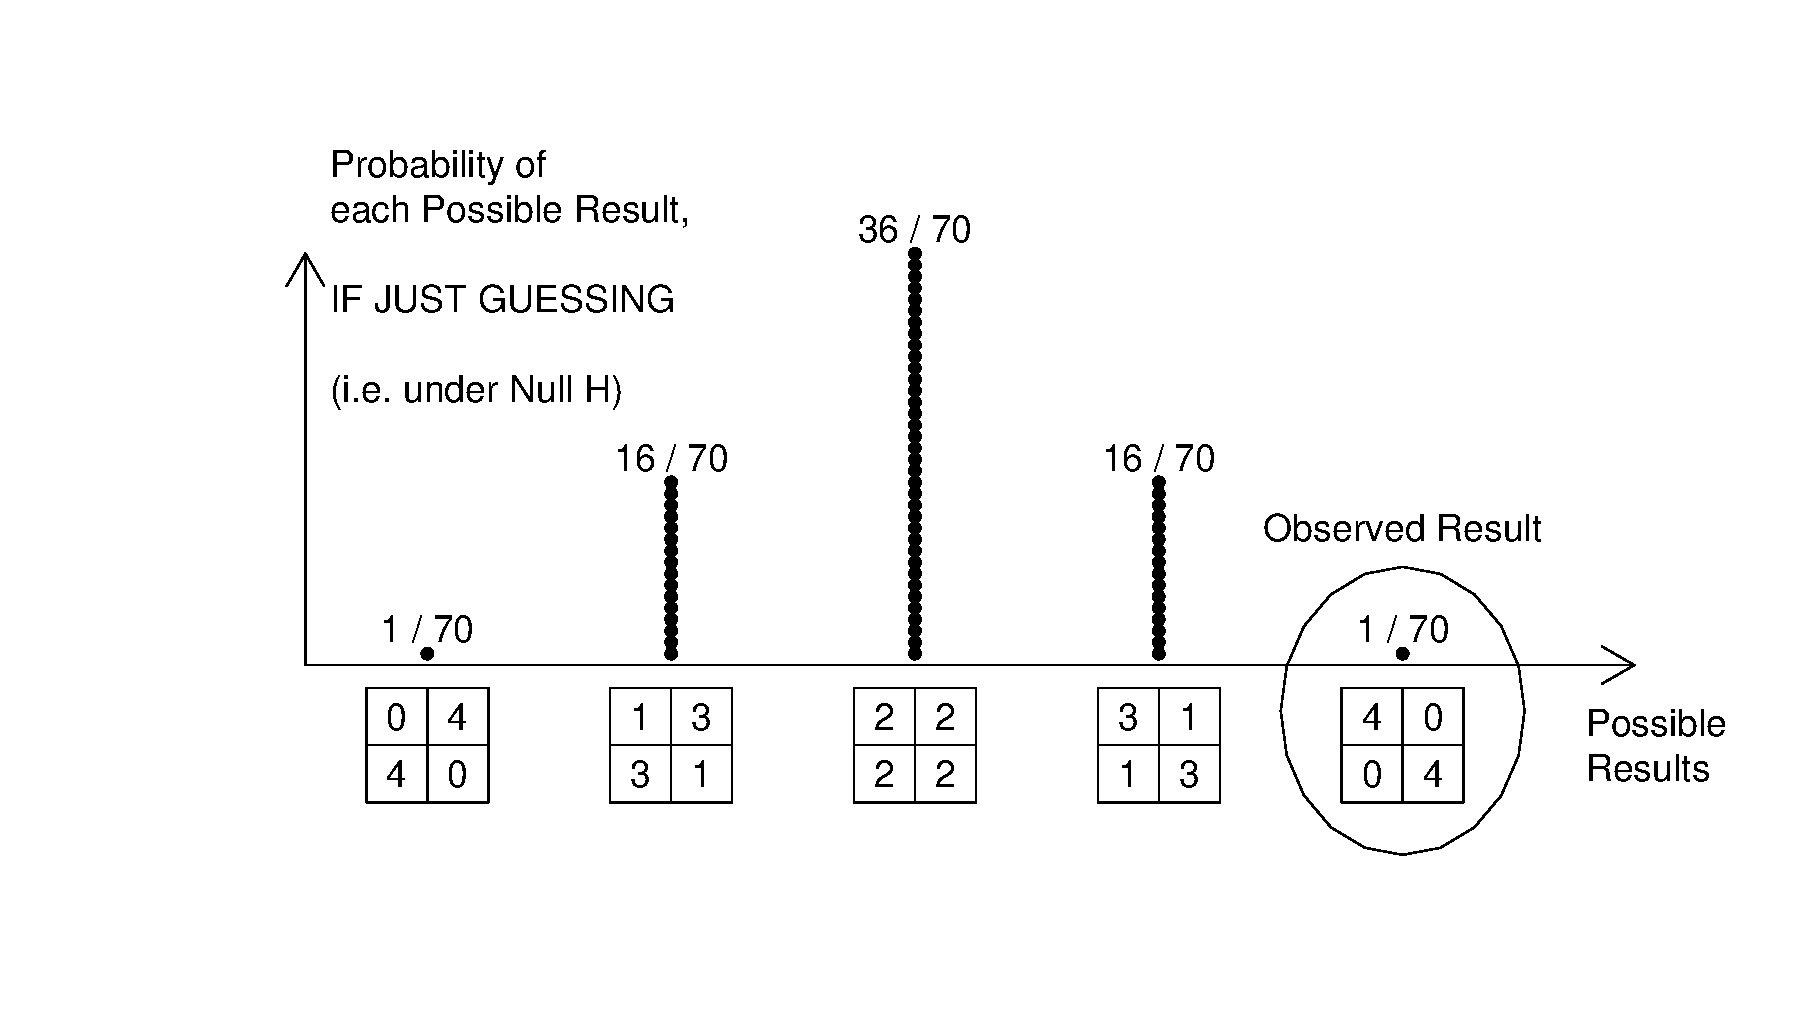
\includegraphics[width=2.5in]{ProbResults.pdf}
			\end{center}
			\pause
			In this example, observed result is the most extreme, so
			$$P_{value}=\textrm{Prob[correctly identifying all 4, IF merely guessing]} = 1/70 = 0.014.$$ \pause
			\item
			Interpretation of such data  often  rather simplistic, as if these \textit{data alone} should \textit{decide}:  i.e. if $P_{value} < 0.05,$ we \sout{`reject' H}$_{null}$; if $P_{value} > 0.05,$ we don't (or worse, we \sout{`accept' H}$_{null}$). Avoid such simplistic `conclusions'.
			
		\end{itemize}
	\end{footnotesize}
\end{frame}

\begin{comment}
\begin{frame}
\frametitle{Example 2 -- Preston-Jones vs. Preston-Jones, English House of Lords, 1949}

\underline{Divorce case:}

\vspace*{.3in}

\begin{itemize}
\item Sole evidence of adultery was that a baby was born almost 50 weeks after husband had gone abroad on military service.  The appeal failed.
\item To quote the court: 
\begin{itemize}
\item ``\textit{The appeal judges agreed that the limit of credibility had to be drawn somewhere, but on medical 
evidence 349 (days) while improbable, was scientifically possible.}''
\end{itemize}
\end{itemize}



\end{frame}

\begin{frame}
\frametitle{Example 2 -- data collected from the 1970s}

\begin{center}
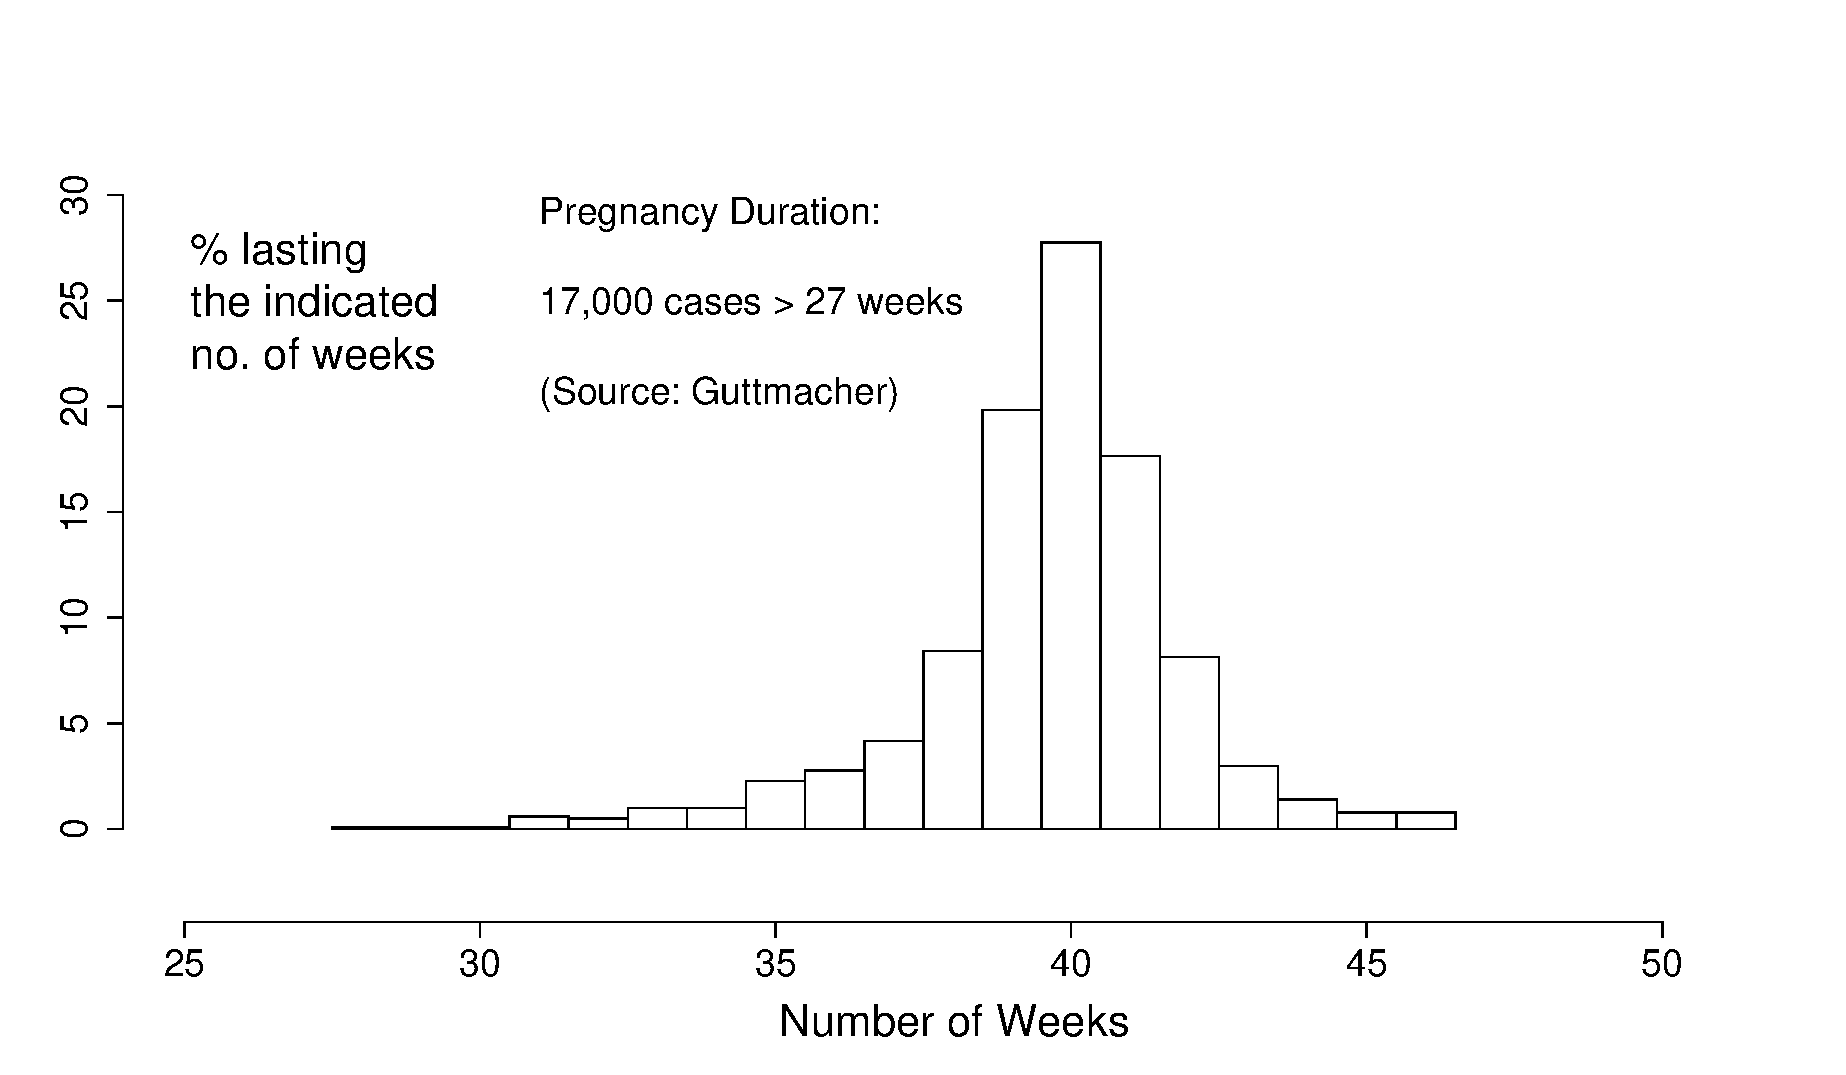
\includegraphics[width=3in]{PregnancyDuration.pdf}
\end{center}

\begin{itemize}
\setlength\itemsep{.3em}
\item $p$-value, calculated under ``Null'' assumption 
that husband was father,  =  `tail area' or probability corresponding  to an observation
of `50 or more weeks' in  above distribution 

%\item Effectively asking: \textbf{What \% of reference distribution does observed value exceed?} \pause 
\item Same system used to report how extreme a lab value is -- are told
where value is located in distribution of values from  healthy (reference) population.
\end{itemize} 


\end{frame}
\end{comment}


\begin{frame}
	\frametitle{$p$-value via the Normal (Gaussian) distribution.}
	
	\begin{footnotesize}
		\begin{itemize}
			\item When judging extremeness of a sample mean or proportion (or  difference between 2 sample means or proportions) calculated from an amount of information that is sufficient for the Central Limit Theorem to apply, one can use Gaussian distribution to readily obtain the $p$-value.
			\item Calculate how many standard errors of the statistic, $SE_{statistic},$ the statistic is from where null hypothesis states true value should be.  This ``number of SE's'' is in this situation referred to as a `$Z_{value}$.'
			$$Z_{value} = \frac{statistic -  \textrm{its expected value under } H_{null} }{SE_{statistic}}.$$
			$p$-value can then be obtained by determining what \% of values in a Normal distribution are as extreme or more extreme than this $Z_{value}.$
			\item
			If $n$ is small enough that value of $SE_{statistic},$ is itself subject to some 
			uncertainty, one would instead refer the ``number of SE's'' to a more appropriate reference distribution, such as Student's $t$- distribution.
		\end{itemize}
		
	\end{footnotesize}
\end{frame}

\begin{frame}
	\frametitle{More about the $p$-value}
	
	%\begin{footnotesize}
	\begin{itemize}
		\setlength\itemsep{.3em}
		\item The $p$-value is a \textbf{probability concerning data}, \textbf{conditional on the Null Hypothesis being true}. \pause
		\item \textbf{Naive (and not so naive) end-users sometimes interpret the $p$-value  as
			the probability that Null Hypothesis is true}, \textit{conditional on -- i.e. given --  the data.} \pause
		%\item Very few MDs mix up complement of specificity (i.e. probability of a `positive'  test result when in fact patient does not have disease in question) with positive predictive value (i.e. probability that a patient who has had a `positive'  test result does  have disease in question).
		\begin{align*}
		p_{value} & = P(\textrm{this or more extreme data}| H_0) \\
		& \neq P(H_0|\textrm{this or more extreme data}).
		\end{align*}
		\item Statistical tests are often coded as statistically significant or not according to whether results are extreme or not with respect to a reference (null)  distribution.  But a test result  is just one piece of data, and needs to be considered \textit{along with  rest of evidence} before coming to a `conclusion.' \item \textbf{Likewise with statistical `tests': the $p$-value is just one more piece of \textit{evidence}, hardly enough to `conclude' anything}. 
		%\item The probability that the DNA from the blood  of a randomly selected (innocent) person would match that from blood on crime-scene glove was 
		%$p=10^{-17}$. \textit{Do not equate this} Prob[data $|$ innocent] \textit{with its transpose}:
		%writing ``data'' as shorthand for ``this or more extreme data'', we need to be aware that 
		%$$p_{value} = Prob[ \ data \  | \  H_0 ] \neq Prob[ \ H_0 \  |  \ data ].$$
	\end{itemize}
	%\end{footnotesize}
\end{frame}

\begin{frame}
	\frametitle{The prosecutor's fallacy \footnote{{\tiny Who's the DNA fingerprinting pointing at? New Scientist, 1994.01.29, 51-52.}}}
	
	\begin{itemize}
		\setlength\itemsep{1em}
		\item Let's suppose a defendant has been accused of robbery
		\item The null hypothesis is that the defendant is innocent. Instructions to juries are quite explicit about this. 
		\item \textbf{Prosecutor}: ``If the defendant were innocent, wouldn't it be remarkable
		that the police found him at the scene of the crime with a bag full of money in
		his hand, a mask on his face, and a getaway car parked outside?'' \mbox{P(innocent $|$ evidence)}
		\item \textbf{Jury}: Considers the evidence in light of the presumption of innocence
		and judges whether the evidence against the defendant would be plausible if
		the defendant were in fact innocent. \mbox{P(evidence $|$ innocent)}
	\end{itemize}
	
\end{frame}

\begin{comment}
\begin{frame}
\frametitle{The prosecutor's fallacy}


\begin{itemize}
\item Statistician Peter Donnelly opened a new area of debate, remarking that 

\begin{itemize}
\setlength\itemsep{1em}
\item \blue{Forensic evidence answers the question}: ``What is the probability that the defendant's DNA profile matches that of the crime sample, assuming that the defendant is innocent?''

\item \blue{While the jury must try to answer the question}: ``What is the probability that the defendant is 		innocent, assuming that the DNA profiles of the defendant and the crime sample match?'' 
\end{itemize}
\pause 
\item
The error in mixing up these two probabilities 
is called ``\textbf{the prosecutor's fallacy},'' 
and it is suggested that newspapers regularly 
make this error. 
\item
Donnelly's testimony convinced the judges 
that the case before them involved an example of this and they 
ordered a retrial.
\end{itemize}

\end{frame}
\end{comment}

\begin{frame}
	\frametitle{The prosecutor's fallacy in a game of poker}
	
	\begin{itemize}
		\setlength\itemsep{1em}
		\item  Imagine the judges were playing a game of poker with the Archbishop of Canterbury. 
		\item If the Archbishop were to deal a royal flush on the first hand, one might suspect him of cheating. \pause 
		\item The probability of the Archbishop dealing a royal flush on any one hand, assuming he is an honest card player, is P(royal flush | innocent) = 1 in 70 000. \pause 
		\item But if the judges were asked whether the Archbishop was honest, given that he had just dealt a royal flush, they would be likely to quote a probability greater than 1 in 70 000 $\to$ P(innocent $|$ royal flush). 
	\end{itemize}
	
\end{frame}


\begin{frame}
	\frametitle{(Intimate) Relationship between $p$-value and CI}
	\begin{center}
		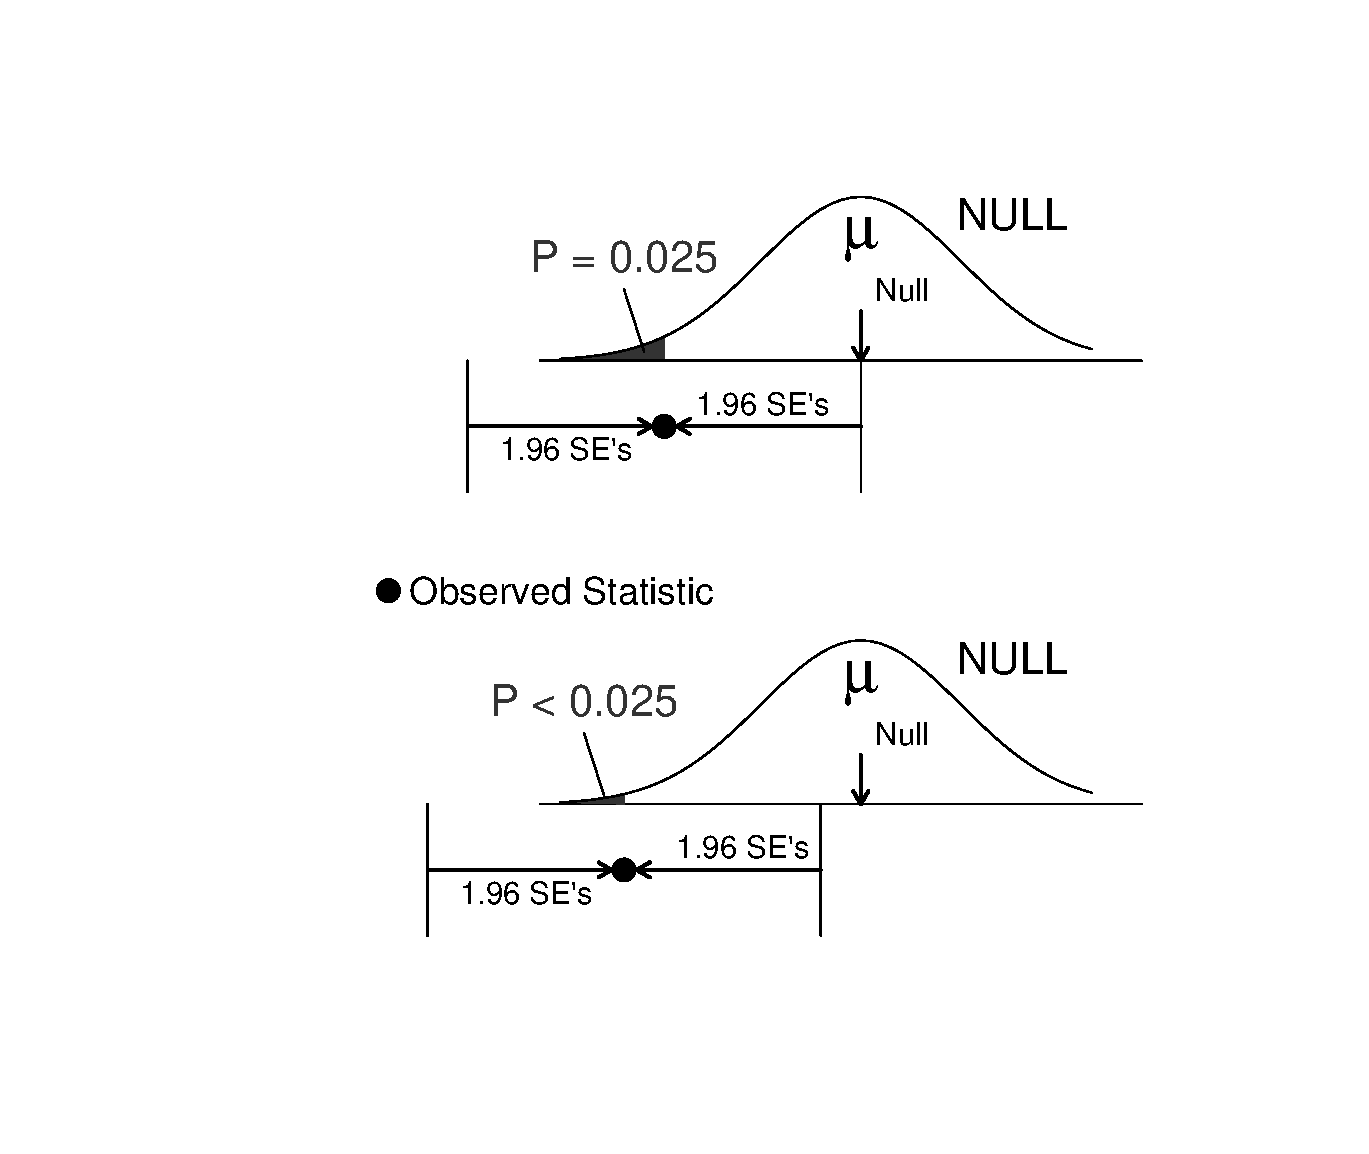
\includegraphics[width=1.65in]{P-CI.pdf}
	\end{center} 
	\begin{footnotesize}
		\begin{itemize}
			\item
			(Upper graph) If upper limit of 95\% CI\textit{ just touches} null value, then
			the 2 sided $p$-value is 0.05 (or 1 sided $p$-value is 0.025). \pause
			\item
			(Lower graph) If upper limit \textit{excludes} null value, then
			the 2 sided $p$-value is less than 0.05 (or 1 sided $p$-value is less than 0.025). \pause
			\item
			(Graph not shown) If  CI \textit{includes} null value, then the 2-sided $p$-value is greater than (the conventional) 0.05, and thus observed statistic is ``not statistically significantly different'' from hypothesized null value. 
		\end{itemize}
	\end{footnotesize}
\end{frame}

\begin{frame}
	\frametitle{Don't be overly-impressed by $p$-values}
	\begin{itemize}
		\setlength\itemsep{0.5em}
		\item
		$p$-values and `significance tests' widely misunderstood and misused.
		\item
		Very large or very small $n$'s can influence what is or is not `statistically significant.'
		\item
		Use CI's instead.
		\item
		\textit{Pre study} power calculations (the chance that results will be `statistically significant', as a
		function of the true underlying difference) of some help.
		\item
		\textit{post-study} (i.e., \textit{after the data have `spoken'}), a CI is much more relevant,
		as it focuses on magnitude \& precision, not on a probability calculated under H$_{null}.$
	\end{itemize}
\end{frame}

\section{Applications}


\begin{frame}
	\frametitle{Do infant formula samples $\downarrow$ dur$^{n.}$ of breastfeeding?\footnote{{\footnotesize Bergevin Y, Dougherty C, Kramer MS. Lancet. 1983 1(8334):1148-51}}}
	
	
	
	Randomized Clinical Trial (RCT) which withheld free formula samples [given by baby-food companies to breast-feeding mothers leaving Montreal General Hospital with their newborn infants] from a random half of those studied.
	
	\begin{scriptsize}
		\begin{center}
			\begin{tabular}{|c c c c c| l|}
				\hline
				& \multicolumn{2}{c}{Mothers}  & & & \\
				At 1 month & given & not given & Total  & $ \ $ &  \\
				& sample & sample & & & \textbf{Conclusion...} \\ 
				\hline
				Still Breast & 175 & 182 & 357 & & \\ 
				feeding & (\textbf{\textit{77\%}}) & (\textbf{\textit{84\%}}) & (80.4\%) & 
				& P=0.07. So, ...  \\ 
				& & & & & the difference is   \\
				Not Breast & 52 & 35 & 87  &  &  ``Not Statistically \\ 
				feeding &  & & & &  Significant" at 0.05 level  \\
				\hline
				Total & 227 & 217 &  444 & & \\
				\hline
			\end{tabular}
		\end{center}
	\end{scriptsize}
	
	\begin{center}
		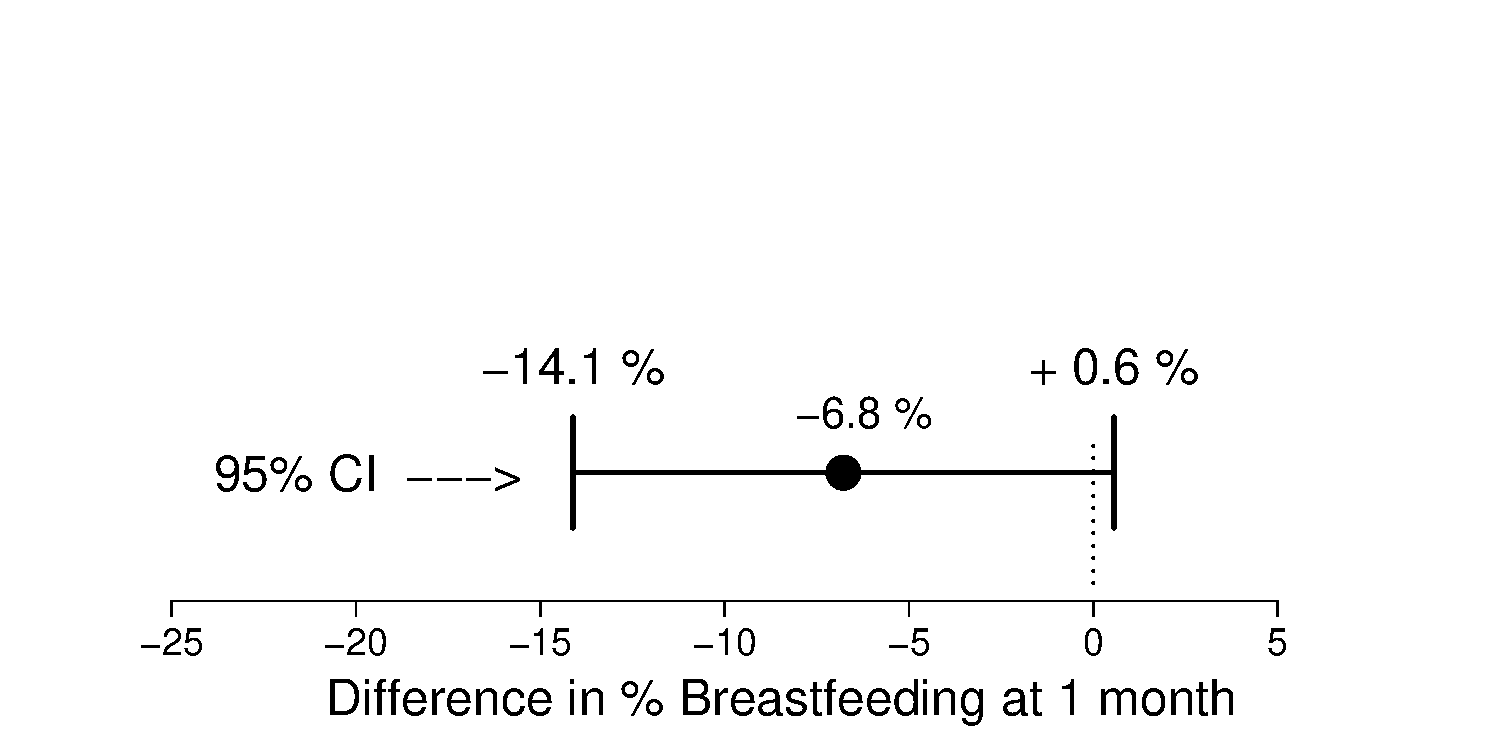
\includegraphics[width=1.75in]{Bergevin.pdf}
	\end{center}
	
\end{frame}

\begin{frame}
	\frametitle{Messages}
	
	\begin{small}
		\begin{itemize}
			\setlength\itemsep{0.5em}
			
			\item \lowercase{NO MATTER WHETHER THE $p$-value IS ``STATISTICALLY SIGNIFICANT'' OR NOT,
				ALWAYS LOOK AT THE LOCATION AND WIDTH OF THE CONFIDENCE INTERVAL. IT
				GIVES YOU A BETTER AND MORE COMPLETE INDICATION OF THE MAGNITUDE OF
				THE EFFECT AND OF THE PRECISION WITH WHICH IT WAS MEASURED.
				\item
				THIS IS AN EXAMPLE OF AN \textbf{INCONCLUSIVE NEGATIVE} STUDY, SINCE IT 
				HAS \textbf{INSUFFICIENT PRECISION} (``RESOLVING POWER") \textbf{TO DISTINGUISH} BETWEEN TWO IMPORTANT POSSIBILITIES -- \textbf{NO HARM}, AND WHAT AUTHOROTIES WOULD CONSIDER A \textbf{SUBSTANTIAL HARM: A REDUCTION OF 10 PERCENTAGE POINTS} IN BREASTFEEDING RATES . 
				\item
				``\textbf{STATISTICALLY} SIGNIFICANT`` AND ``\textbf{CLINICALLY}-'' (OR ``\textbf{PUBLIC HEALTH}-'') SIGNIFICANT ARE DIFFERENT CONCEPTS.   
				
				\item
				(Message from 1st author:) Plan to have \textbf{enough statistical power}. His study had only 50\% power to detect a difference of 10 percentage points)}
			
		\end{itemize}
	\end{small}
\end{frame}

\begin{frame}
	\frametitle{Do starch blockers really block calorie absorption?}
	
	{\scriptsize Starch blockers -- their effect on calorie absorption from a high-starch meal.
		Bo-Linn GW. et al New Eng J Med. 307(23):1413-6, 1982 Dec 2}
	
	\begin{footnotesize}
		
		\begin{itemize}
			\item
			Known for more than 25 years that certain plant foods, e.g., kidney beans \& wheat, contain a substance that inhibits activity of salivary and pancreatic amylase.
			\item
			More recently, this antiamylase has been purified and marketed for use in weight control under generic name ``starch blockers.'' 
			\item
			Although this approach to weight control is highly popular, it has never been shown whether starch-blocker tablets actually reduce  absorption of calories from starch.
			\item
			Using a one-day calorie-balance technique and a high starch (100 g) meal (spaghetti, tomato sauce, and bread), we measured excretion of fecal calories after $n=5$ normal subjects in a cross-over trial had taken either placebo or starch-blocker tablets.
			\item
			If the starch-blocker tablets had prevented the digestion of starch, fecal calorie excretion should have increased by 400 kcal.
		\end{itemize}
	\end{footnotesize}
\end{frame}

\begin{frame}
	\frametitle{Do starch blockers really block calorie absorption?}
	
	\begin{itemize}
		\item
		However, fecal calorie excretion was same on the 2 test days (mean $\pm$ S.E.M., 80 $\pm$ 4 as compared with 78 $\pm$ 2).
		\begin{center}
			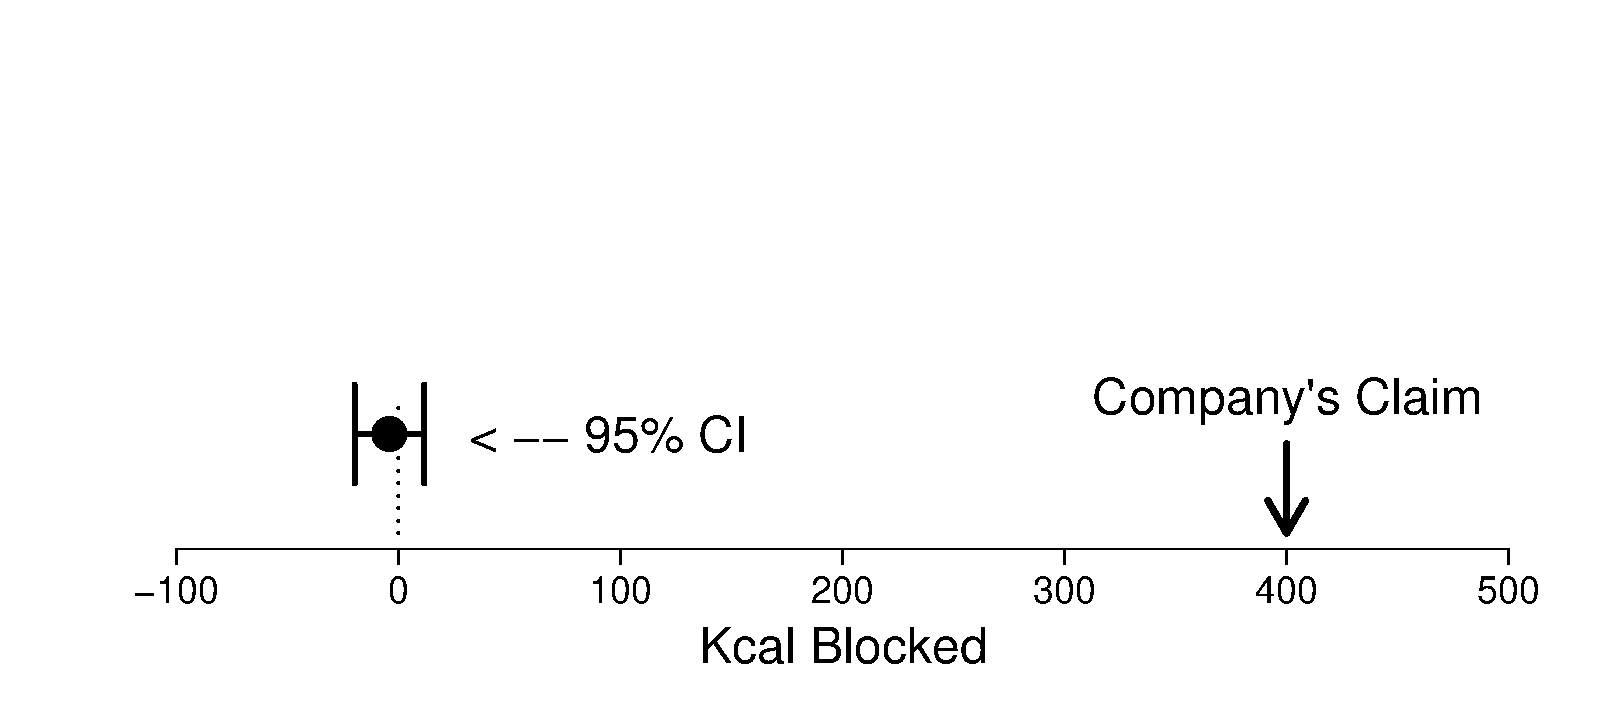
\includegraphics[width=4in]{StarchBlockers.pdf}
		\end{center}
		\item
		We conclude that starch blocker tablets do not inhibit the digestion and absorption of starch calories in human beings.
		\item
		EFFECT IS MINISCULE (AND ESTIMATE QUITE PRECISE) 
		AND VERY FAR FROM COMPANY'S CLAIM !!! 
		\item
		A `\textbf{DEFINITIVELY NEGATIVE}' STUDY.
	\end{itemize}
\end{frame}

\section{Summary}
\begin{frame}
	\frametitle{SUMMARY - 1}
	\begin{itemize}
		\setlength\itemsep{1em}
		%\item The difference sources of variability have important implications in patient management.
		%\item Descriptive statistics should be descriptive, and should suit the pattern of variation.
		\item Confidence intervals  preferable to $p$-values, since they are expressed in terms of (comparative) parameter of interest;  they allow us to judge magnitude and its precision, and help  us in
		`ruling in / out'  certain parameter values. 
		\item
		A `statistically significant' difference does not necessarily imply a clinically important difference.
		\item
		A `not-statistically-significant' difference does not necessarily imply that we have ruled out a clinically important difference. 
	\end{itemize}
\end{frame}

\begin{frame}
	\frametitle{SUMMARY - 2}
	\begin{itemize}
		\setlength\itemsep{.51em}
		\item
		Precise estimates  distinguish b/w that which --  if it were true  -- would be important and that which --  if it were true  --  would not. `$n$'  an important determinant of precision.
		\item A lab value in upper 1\% of reference distribution  (of values derived from people  without known diseases/conditions )  does not mean that there is a 1\% chance that person in whom it was measured is healthy; i.e., it doesn't mean that there's a 99\% chance that the person in whom it was measured  does have some disease/condition.
		\item Likewise,  $p$-value $\neq$ probability that null hypothesis is true.
		\item
		The fact that 
		$$Prob[ the \ data \ | \ Healthy ]\textrm{  is small [or large]}$$
		does not necessarily mean that
		$$Prob[ Healthy \ | \ the \ data ]\textrm{  is small [or large]}$$
	\end{itemize}
\end{frame}

\begin{frame}
	\frametitle{SUMMARY - 3}
	\begin{itemize}
		\item
		Ultimately, $p$-values, CI's and other evidence from a study need to be combined with other information bearing on  parameter or process. \newline
		\item
		Don't treat any one study as last word on the topic. \newline
		%\item
		%Worry also about distortions of a non-sampling kind that are not minimized by having a large `$n$.' A larger sample size will not reduce  systematic differences in a comparison. \newline
	\end{itemize}
\end{frame}




\end{document}
